Com o progresso do projeto, alcançamos os seguintes resultados: a prototipação das telas para dispositivos móveis utilizando o software Figma, a construção do site com a ferramenta Oracle APEX (uma plataforma que facilita o desenvolvimento de aplicações web), a elaboração do Diagrama de Caso de Uso (DCU), a Modelagem do Banco de Dados (MBD), tanto na perspectiva lógica quanto conceitual, a definição do Escopo de Redes e a criação do Modelo de Negócios no Canvas Sebrae.

\textbf{Prototipação do Aplicativo}

Com ajuda do Figma fizemos a primeira tela, que é chamada de Splash Screen (tela inicial), nela voce o usuário pode cadastrar uma conta ou entrar com uma conta já existente conforme ilustrado na \Cref{phot:pg-2}.

\begin{figure}[H]
    \centering
    \SetCaptionWidth{\ifbool{@LayoutA}{0.6}{0.72}\linewidth}
    \caption{Splash Screen}%
    \label{phot:pg-2}
    \savebox0{
\includegraphics[scale=0.5]{Illustrations/Login.jpg}}
    \usebox0%
    \SourceOrNote{Autoria Própria (2024)}
\end{figure}

    Já na tela principal do aplicativo o usuário pode escolher três funções interativas principais através de uma tela rolável, sendo elas: Escanear Folha, Meus Arquivos e Indices Locais como mostrado na   \Cref{phot:pg-3}.

    \begin{figure}[H]
        \centering
        \SetCaptionWidth{\ifbool{@LayoutA}{0.6}{0.72}\linewidth}
        \caption{Main Screen (Tela Principal)}%
        \label{phot:pg-3}
        \savebox0{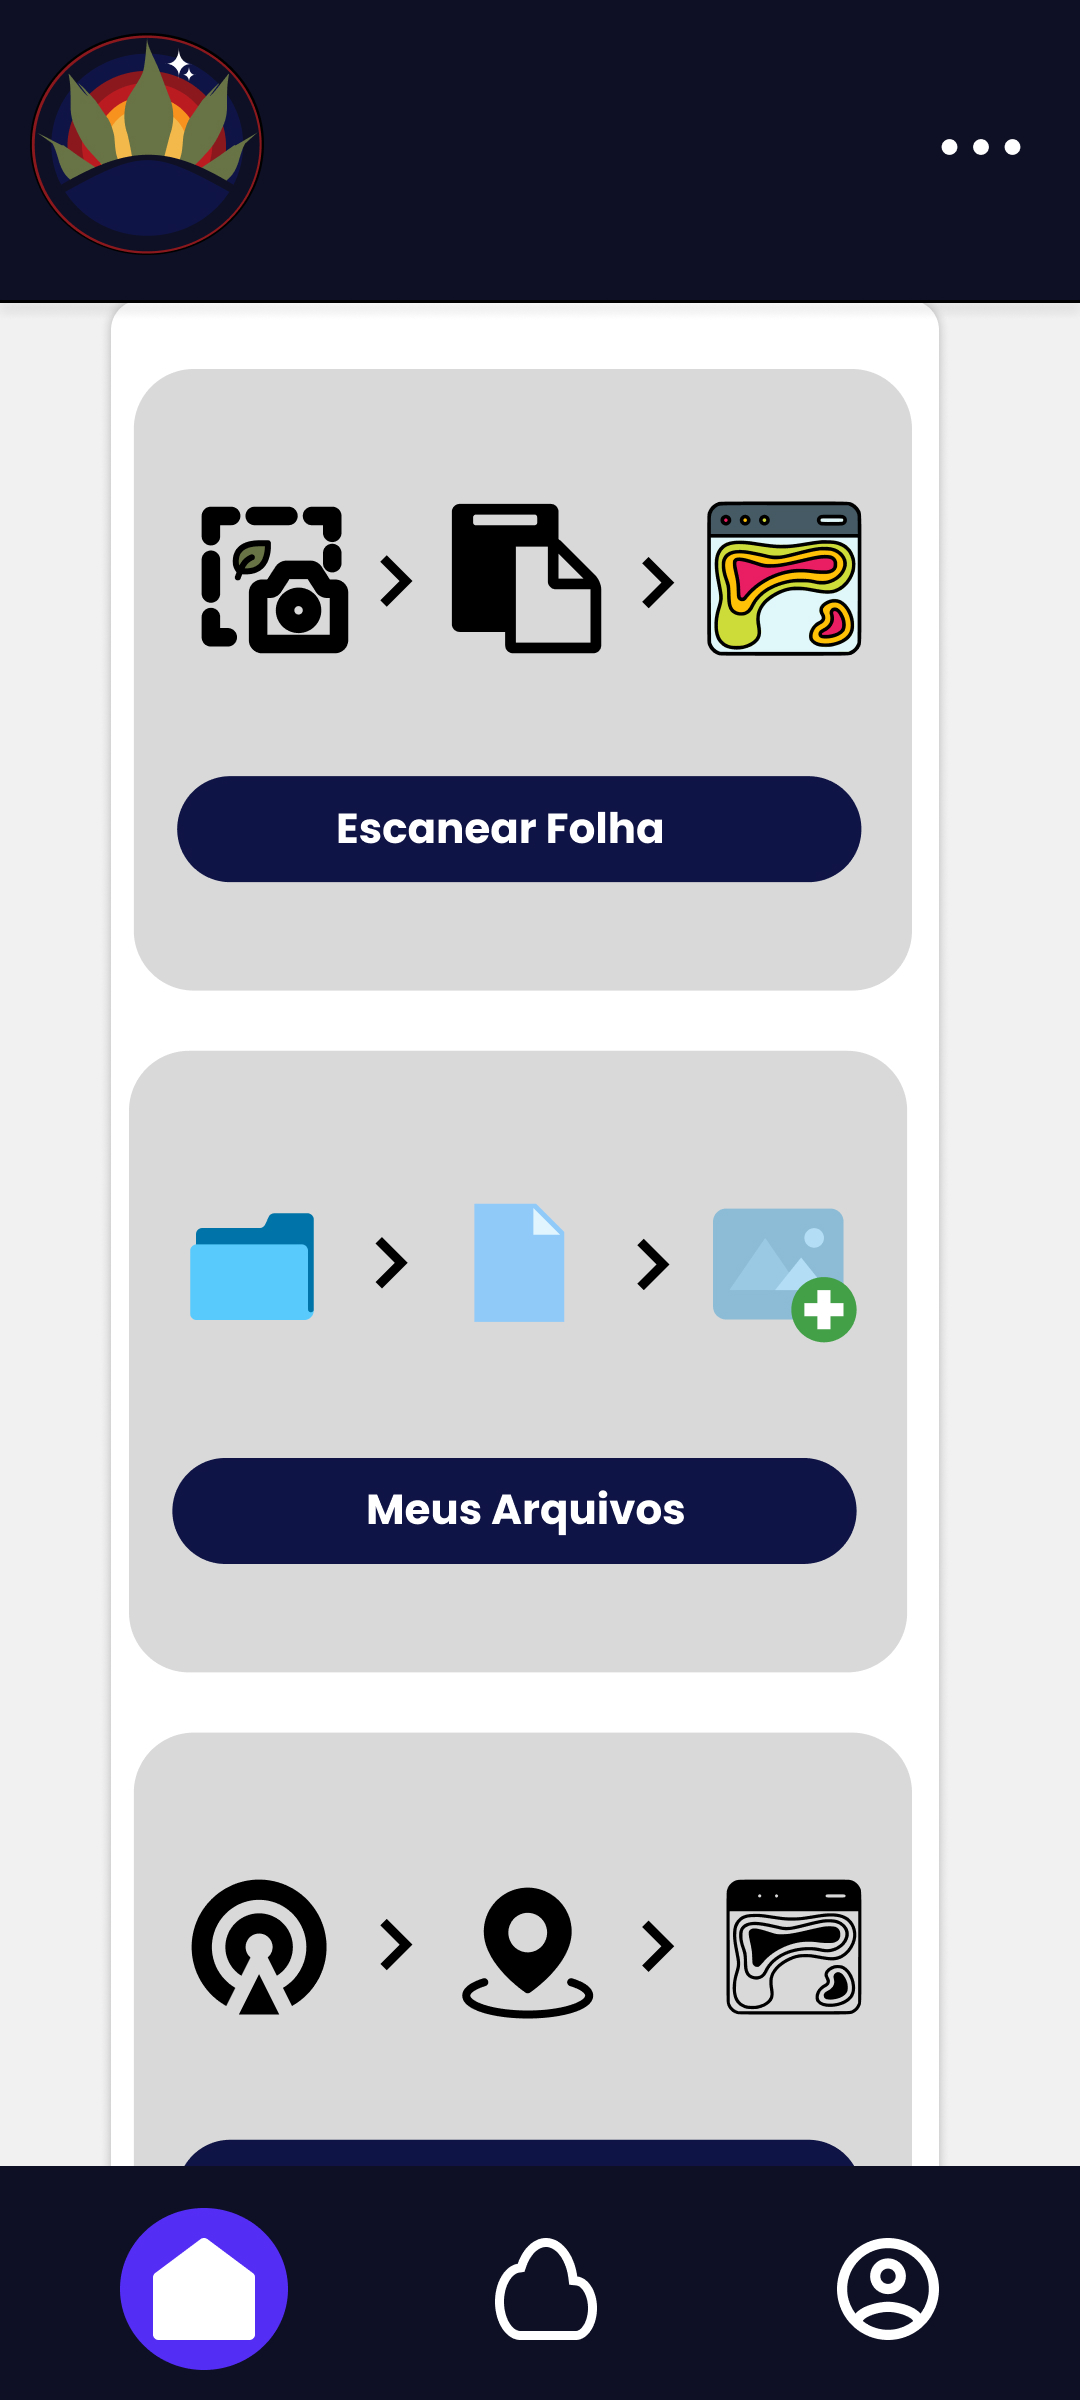
\includegraphics[scale=0.5]{Illustrations/PRINCIPAL.jpg}}
        \usebox0%
        \SourceOrNote{Autoria Própria (2024)}
    \end{figure}

    Após apertar para Escanear a folha o aplicativo leva o usuário para tela de escaneamento, onde uma Inteligência Artificial analisa a imagem tirada pelo usuário \Cref{phot:pg-4}.   

    \begin{figure}[H]
        \centering
        \SetCaptionWidth{\ifbool{@LayoutA}{0.6}{0.72}\linewidth}
        \caption{Tela de Escaneamento (Scan Screen)}%
        \label{phot:pg-4}
        \savebox0{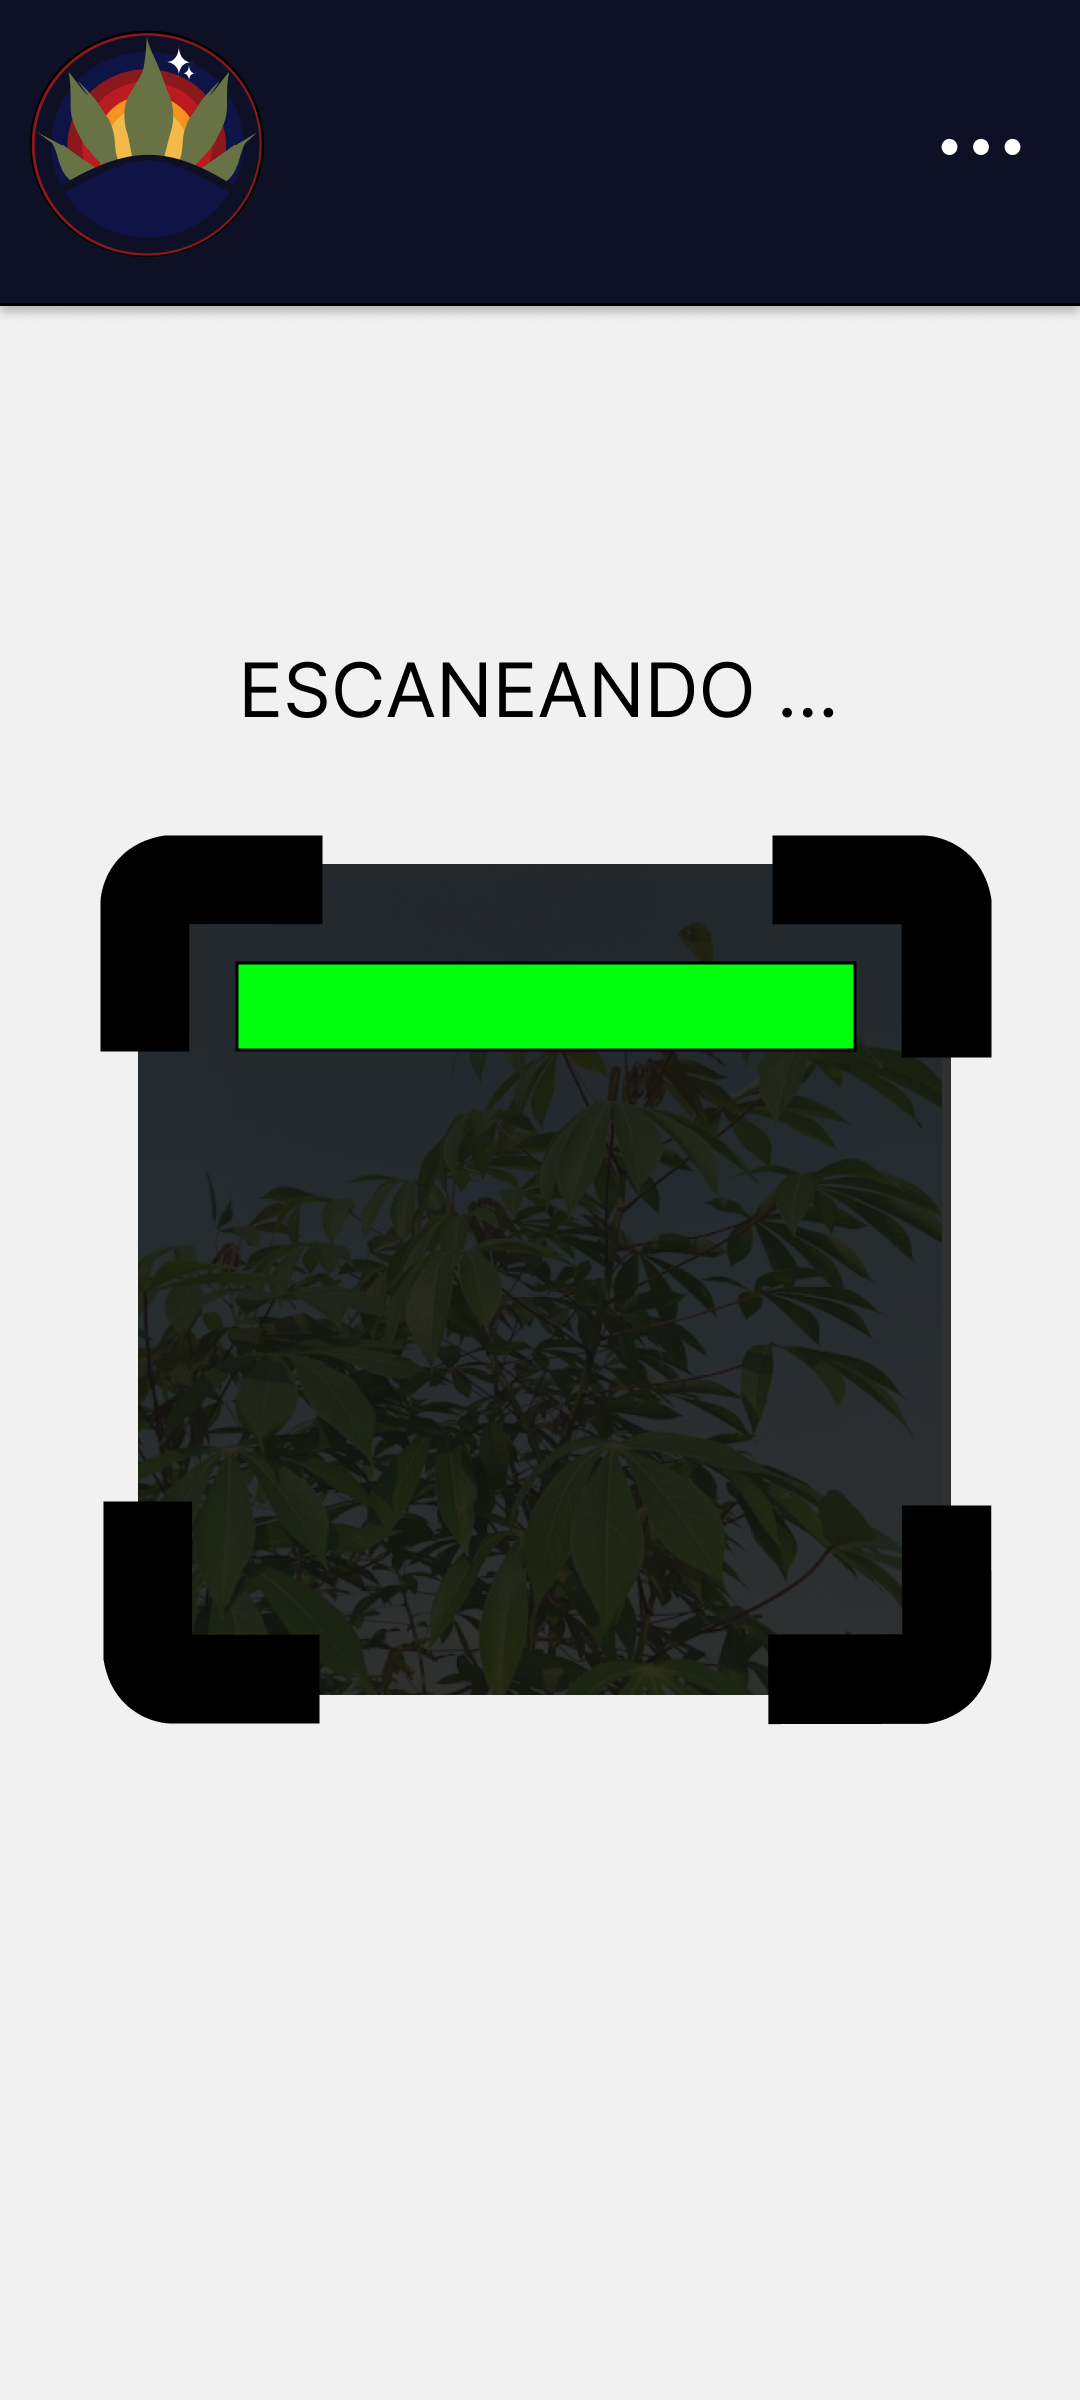
\includegraphics[scale=0.5]{Illustrations/Identificacao.png}}
        \usebox0%
        \SourceOrNote{Autoria Própria (2024)}
    \end{figure}

    Em seguida é mostrado na tela a probabilidade da folha da mandioca possuir a bacteriose, em uma seção onde é mostrado em detalhes o que aconteceu com a planta com a ajuda da analise fornecida pela IA (Inteligência Artificial); o usuário também pode salvar a sua localização para registrar no mapa de calor da região \Cref{phot:pg-5}.
    \begin{figure}[H]
        \centering
        \SetCaptionWidth{\ifbool{@LayoutA}{0.6}{0.72}\linewidth}
        \caption{Tela Relatório (Report Screen)}%
        \label{phot:pg-5}
        \savebox0{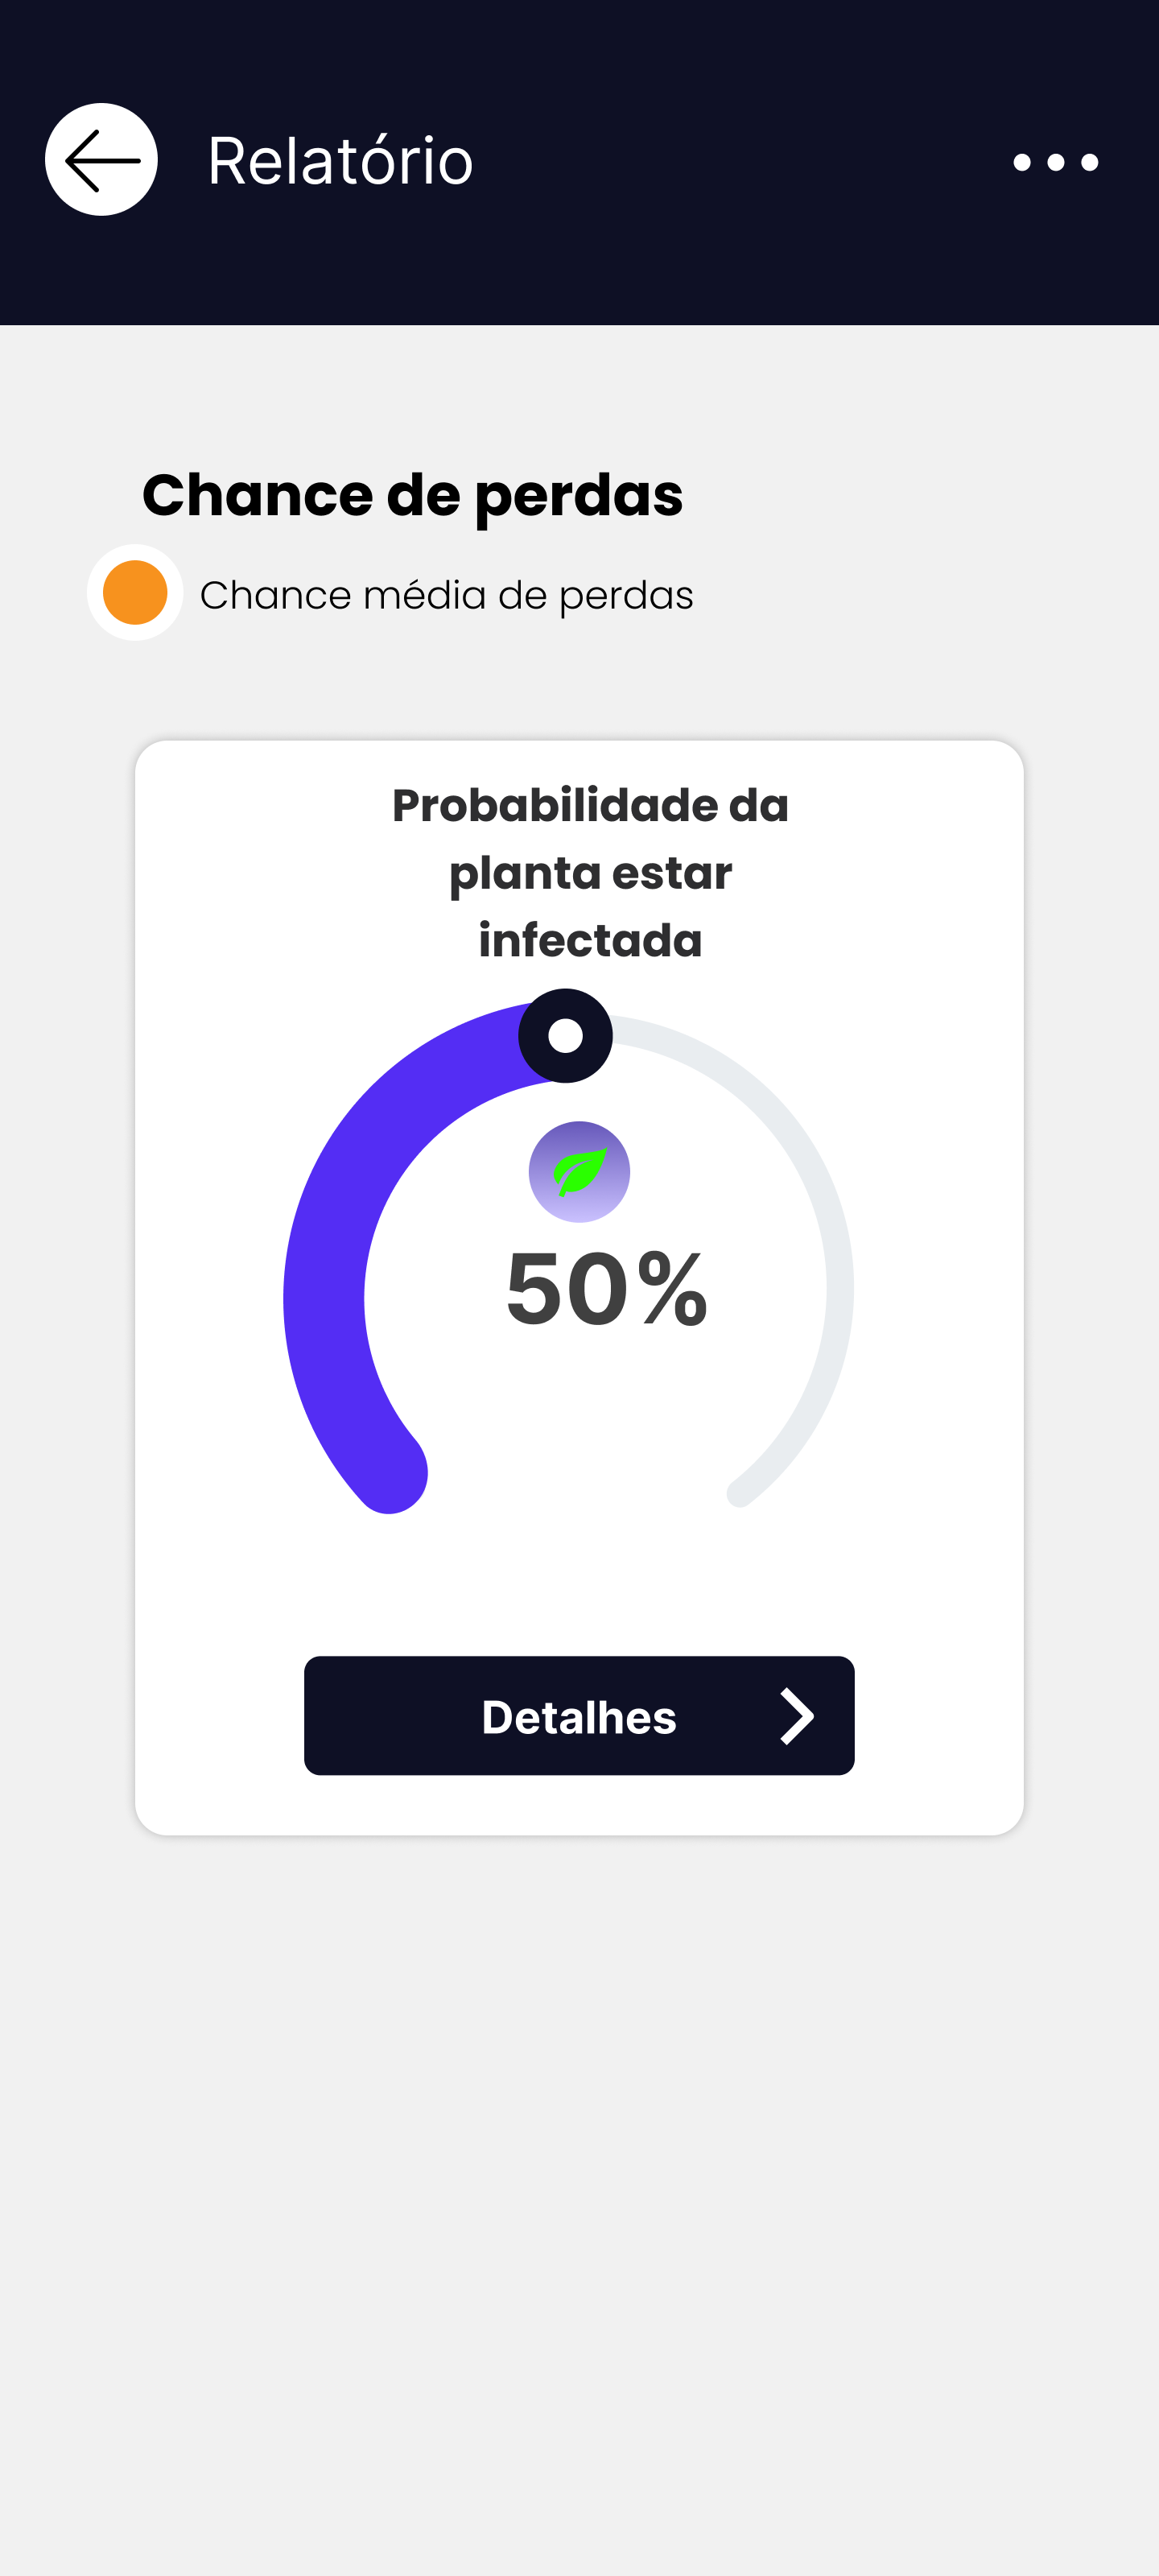
\includegraphics[scale=0.5]{Illustrations/Relatorio_2.png}}
        \usebox0%
        \SourceOrNote{Autoria Própria (2024)}
    \end{figure}

    Após o usuário salvar a imagem no mapa de calor ele é encaminhado para tela de Índices Locais onde será mostrado o mapa de calor da região \Cref{phot:pg-6}.
    
    \begin{figure}[H]
        \centering
        \SetCaptionWidth{\ifbool{@LayoutA}{0.6}{0.72}\linewidth}
        \caption{Mapa de Calor (Heat Map)}%
        \label{phot:pg-6}
        \savebox0{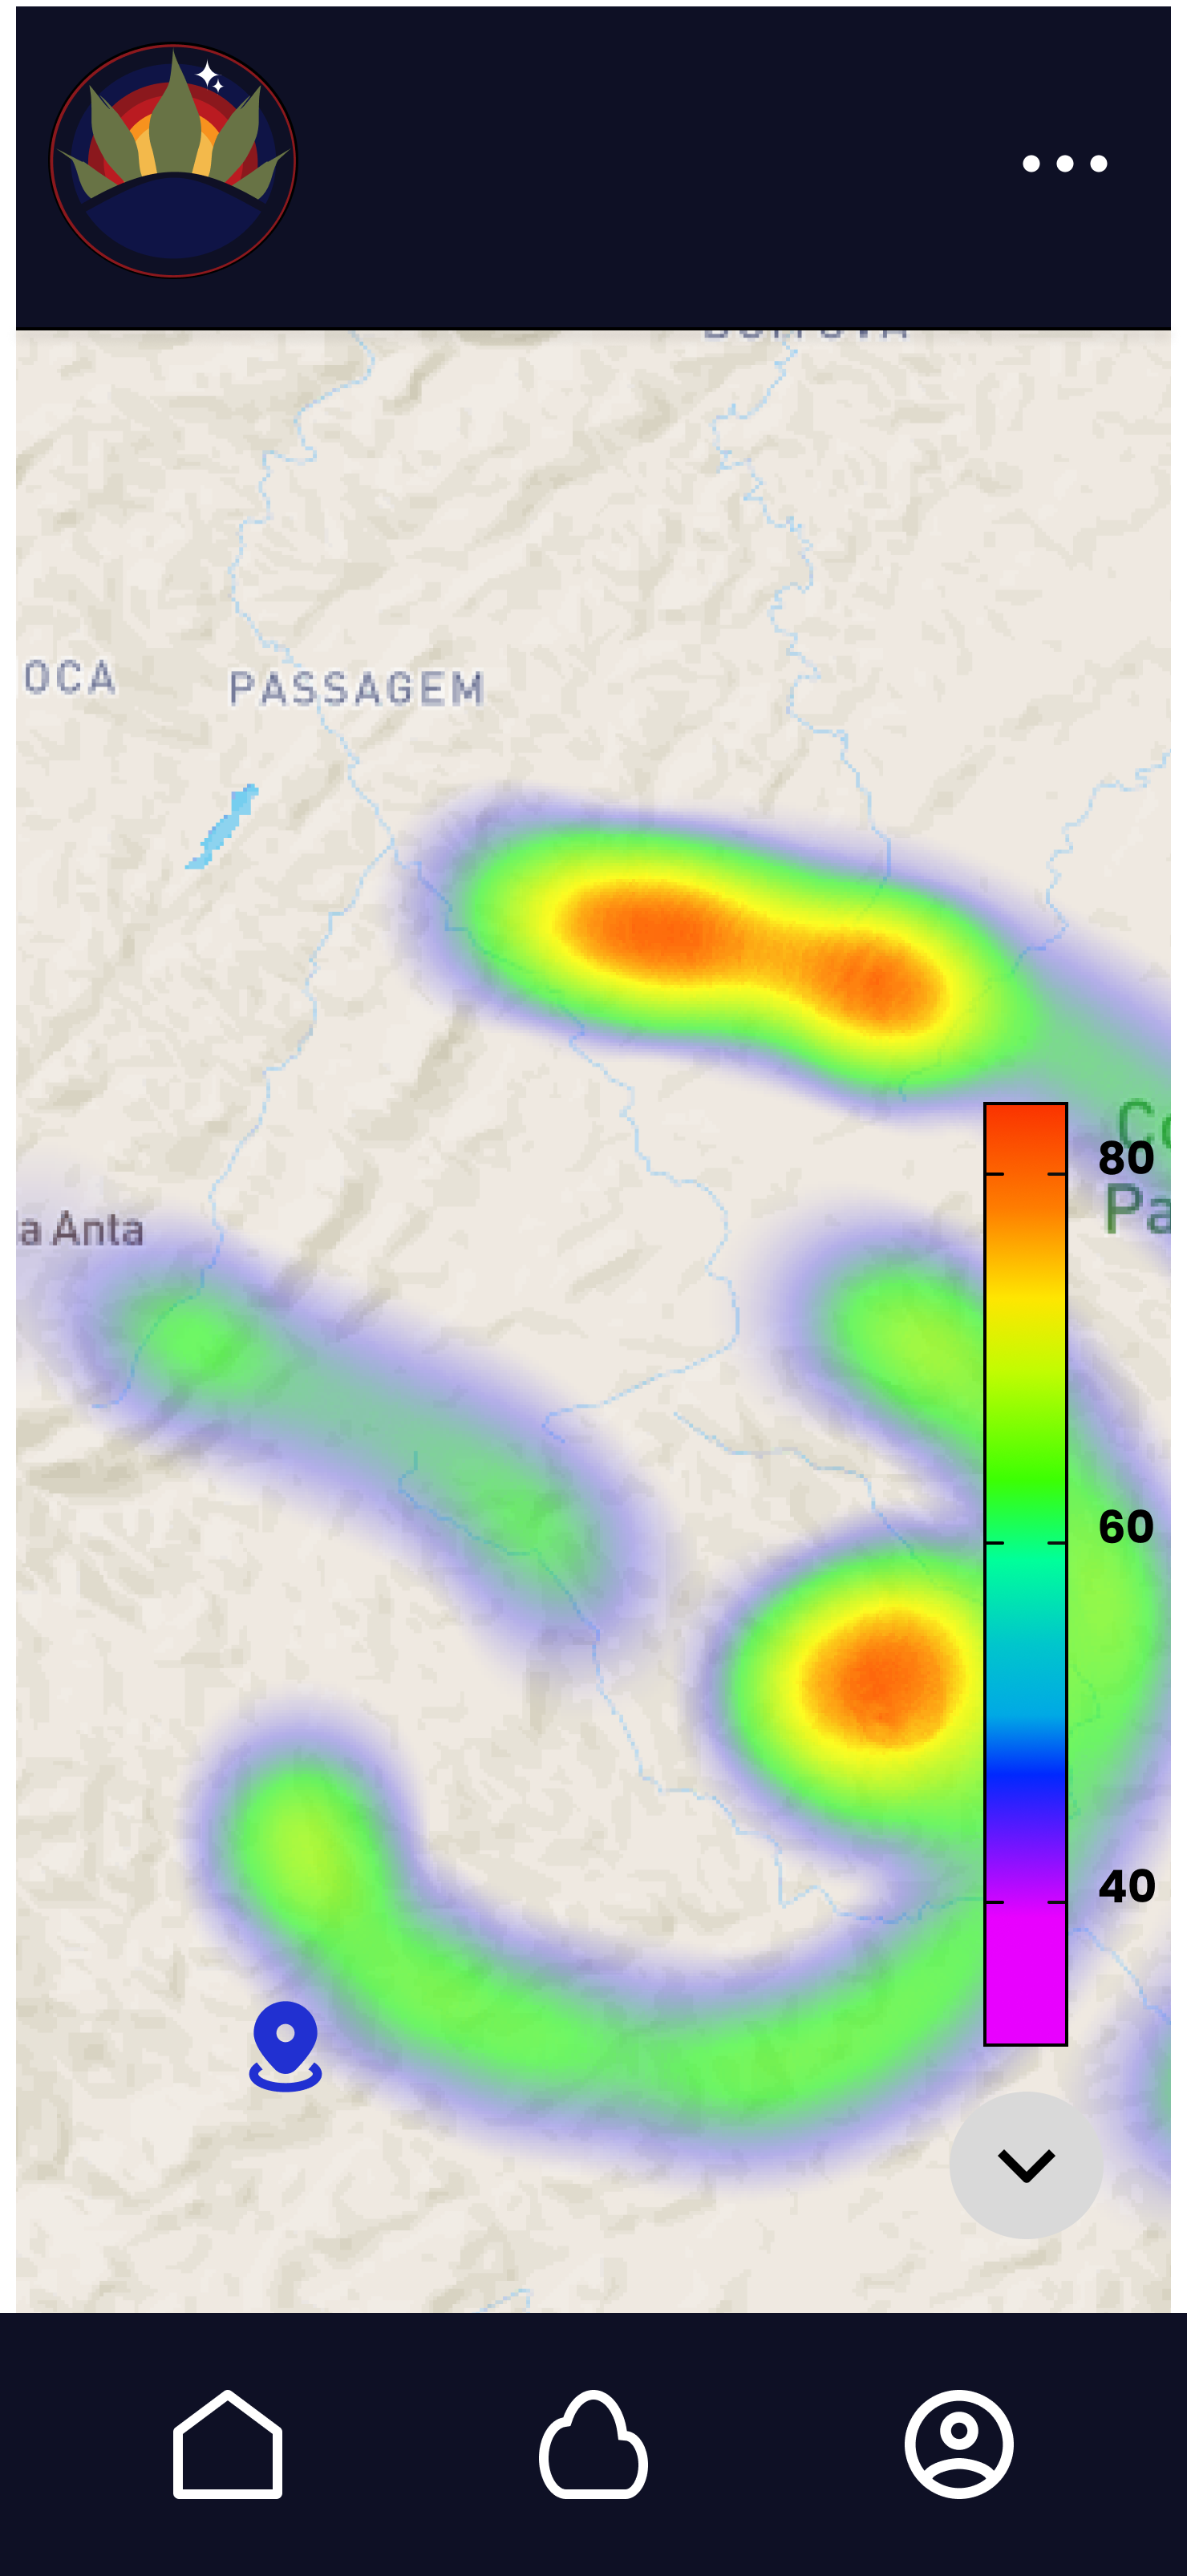
\includegraphics[scale=0.5]{Illustrations/mapa_calor.png}}
        \usebox0%
        \SourceOrNote{Autoria Própria (2024)}
    \end{figure}

    \textbf{APEX}
    
    O APEX é uma plataforma de desenvolvimento da Oracle que possui o intuito de criar aplicativos web de forma rápida e sem necessidade de conhecimentos profundos em programação. O APEX oferece uma interface gráfica para o desenvolvimento de aplicações que integram facilmente com bancos de dados Oracle, ideal para criar painéis, formulários, relatórios, e outras funcionalidades interativas.

    A primeira tela criada no APEX foi a tela de início, que é exibida quando o proprietário acessa o sistema. Essa tela inicial serve como ponto de entrada e fornece uma visão geral do sistema, permitindo uma navegação rápida para as funcionalidades principais, como mostrado na ilustração \Cref{phot:pg-15}.

    \begin{figure}[H]
        \centering
        \SetCaptionWidth{\ifbool{@LayoutA}{0.6}{0.72}\linewidth}
        \caption{Tela de início(APEX)}%
        \label{phot:pg-15}
        \savebox0{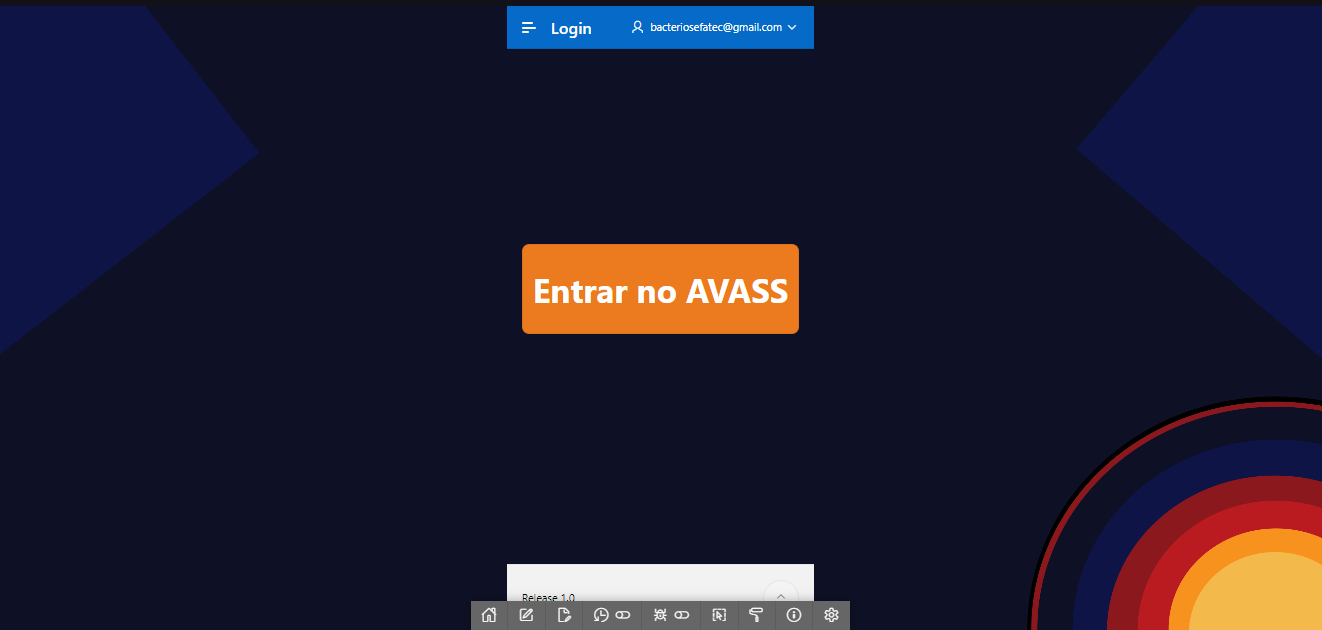
\includegraphics[scale=0.5]{Illustrations/Tela1_APEX.png}}
        \usebox0%
        \SourceOrNote{Autoria Própria (2024)}
    \end{figure}

    Na Figura \Cref{phot:pg-15} é mostrado a tela de login onde o proprietário entra com sua conta.

    \begin{figure}[H]
        \centering
        \SetCaptionWidth{\ifbool{@LayoutA}{0.6}{0.72}\linewidth}
        \caption{Tela de login(APEX)}%
        \label{phot:pg-15}
        \savebox0{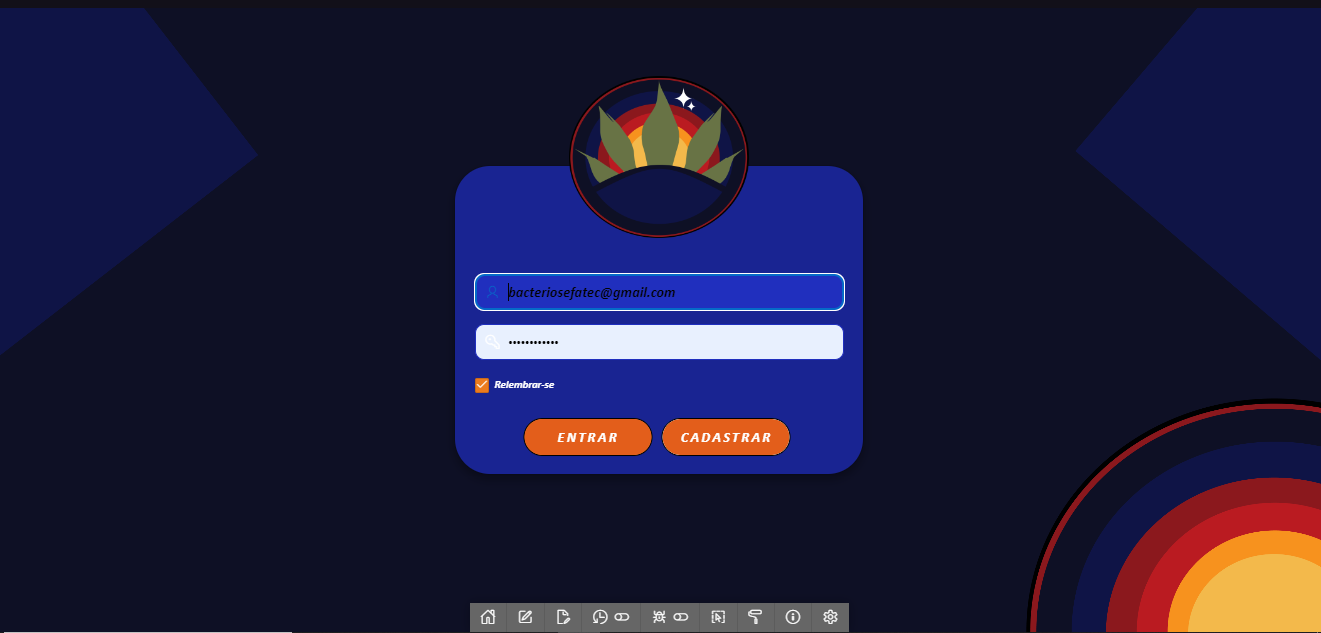
\includegraphics[scale=0.5]{Illustrations/tela2_APEX.png}}
        \usebox0%
        \SourceOrNote{Autoria Própria (2024)}
    \end{figure}

    Após o proprietário entrar, ele é direcionado para a tela do mapa de calor, onde pode visualizar as estatísticas clicando no botão "Ver nas tabelas". \Cref{phot:pg-16}

    
    \begin{figure}[H]
        \centering
        \SetCaptionWidth{\ifbool{@LayoutA}{0.6}{0.72}\linewidth}
        \caption{Mapa de Calor(APEX)}%
        \label{phot:pg-16}
        \savebox0{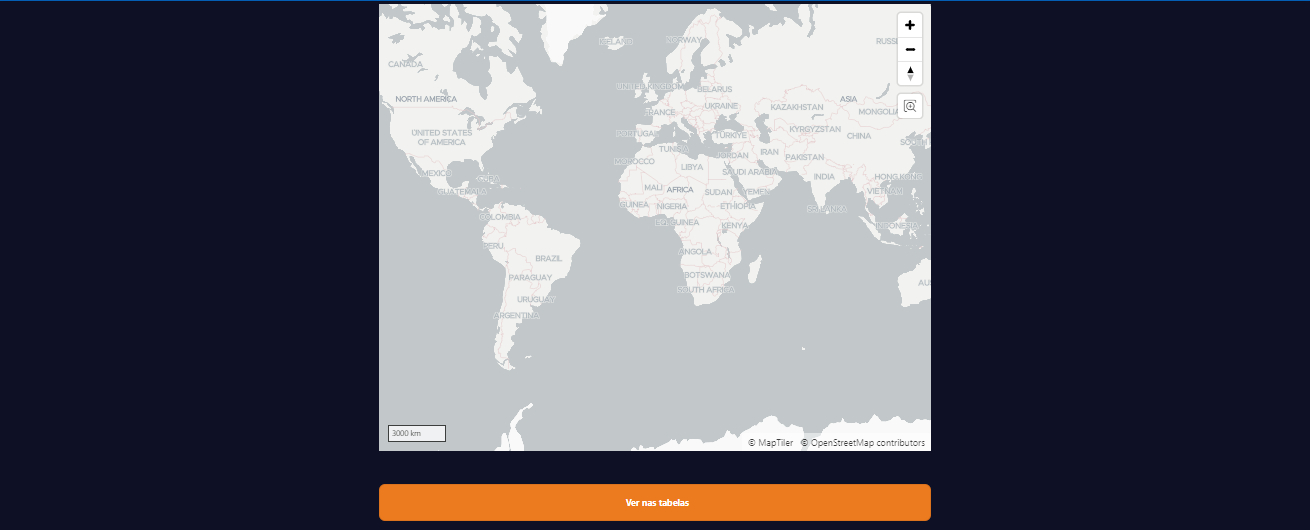
\includegraphics[scale=0.5]{Illustrations/tela3_APEX.png}}
        \usebox0%
        \SourceOrNote{Autoria Própria (2024)}
    \end{figure}

    Ao entrar na tela das Tabelas o usuário pode consultar precisamente a quantidade de plantas infectadas mostradas anteriormente no mapa de calor representado na \Cref{phot:pg-17}.

    \begin{figure}[H]
        \centering
        \SetCaptionWidth{\ifbool{@LayoutA}{0.6}{0.72}\linewidth}
        \caption{Tabelas(APEX)}%
        \label{phot:pg-17}
        \savebox0{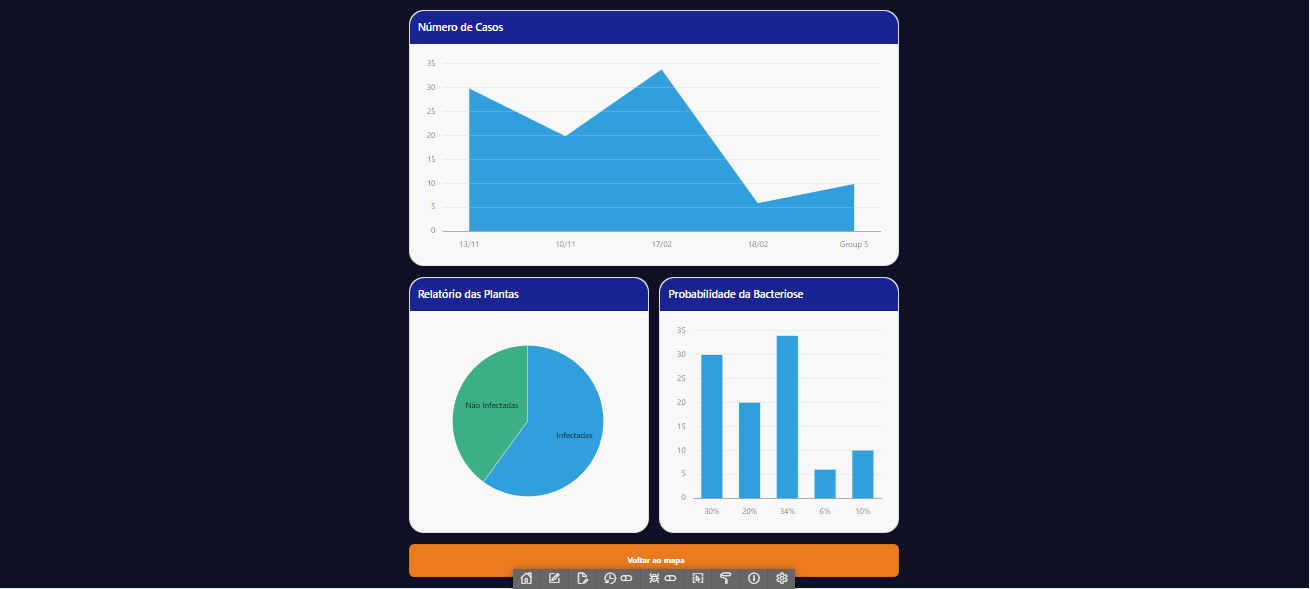
\includegraphics[scale=0.5]{Illustrations/Tela4_APEX.png}}
        \usebox0%
        \SourceOrNote{Autoria Própria (2024)}
    \end{figure}


    \textbf{Diagrama de DCU} 

    Um Diagrama de DCU (ou Diagrama de Casos de Uso) é um tipo de diagrama utilizado na modelagem de sistemas para descrever as interações entre usuários (ou outros sistemas) e o próprio sistema. Seu principal objetivo é demonstrar as diferentes maneiras pelas quais o usuário pode interagir com o sistema, conforme representado na imagem \Cref{phot:pg-12}. Ele faz parte da UML (Unified Modeling Language), uma linguagem de modelagem padrão para representar a estrutura e o comportamento de sistemas de software.

    \begin{figure}[H]
        \centering
        \SetCaptionWidth{\ifbool{@LayoutA}{0.6}{0.72}\linewidth}
        \caption{Diagrama de Caso e Uso (DCU)}%
        \label{phot:pg-12}
        \savebox0{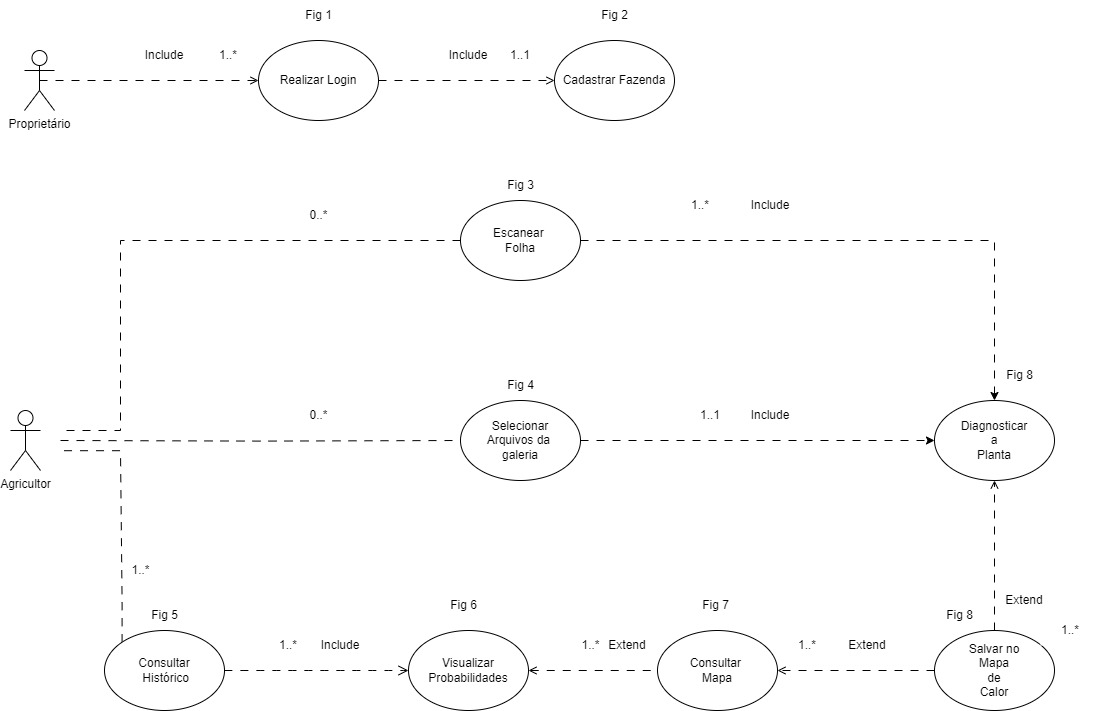
\includegraphics[scale=0.4]{Illustrations/Caso_uso_solo.jpg}}
        \usebox0%
        \SourceOrNote{Autoria Própria (2024)}
    \end{figure}

    \textbf{Modelagem de Banco de Dados (MBD)} \\
    Um modelo relacional é uma abordagem para organizar dados em tabelas, chamadas de relações, onde cada linha representa uma entidade e cada coluna representa um atributo. Ele utiliza chaves primárias para identificar registros de forma única e chaves estrangeiras para estabelecer relações entre as tabelas. Esse modelo é a base dos sistemas de gerenciamento de banco de dados relacionais (SGBD), como mostrado na \Cref{phot:pg-13}. 
    \begin{figure}[H]
        \centering
        \SetCaptionWidth{\ifbool{@LayoutA}{0.6}{0.72}\linewidth}
        \caption{Modelo Conceitual(DCU)}%
        \label{phot:pg-13}
        \savebox0{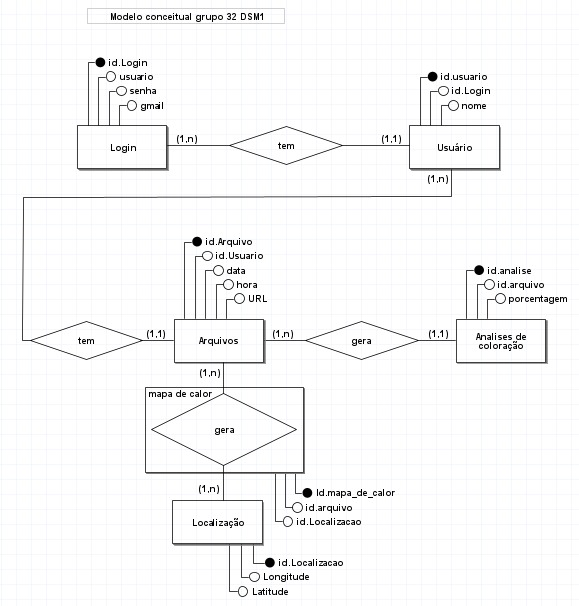
\includegraphics[scale=0.5]{Illustrations/BDC.jpeg}}
        \usebox0%
        \SourceOrNote{Autoria Própria (2024)}
    \end{figure}

    \begin{figure}[H]
        \centering
        \SetCaptionWidth{\ifbool{@LayoutA}{0.6}{0.72}\linewidth}
        \caption{Modelo Lógico(DCU)}%
        \label{phot:pg-14}
        \savebox0{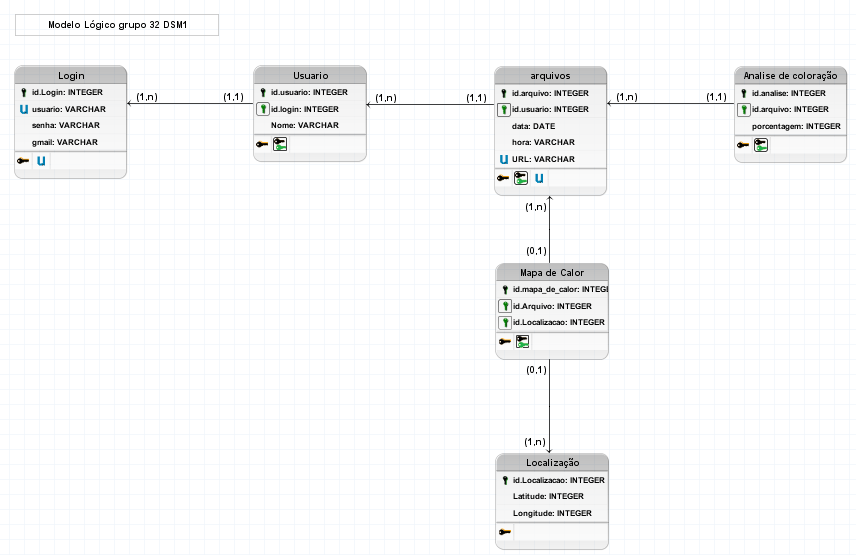
\includegraphics[scale=0.8]{Illustrations/mod_logic1.png}}
        \usebox0%
        \SourceOrNote{Autoria Própria (2024)}
    \end{figure}
    
   Ambos modelos foram criados para mostrar o funcionamento do projeto \textit{Classificação de Bacteriose nas Folhas da Mandioca por Aprendizagem Profunda}, onde o usuário pode tirar fotos, armazená-las e obter uma probabilidade de a planta possuir a bacteriose \textit{Xanthomonas Paesoli}. As entidades \textit{Login} e \textit{Usuário} possibilitam que o usuário entre no sistema. A entidade \textit{Login} possui os seguintes atributos: \textit{id\_login}, como identificador único, \textit{usuario}, como nome do usuário, \textit{senha} e \textit{email}. A entidade \textit{Usuário} possui os atributos: \textit{id\_usuario}, \textit{id\_login} e \textit{nome}. 

    A entidade \textit{Usuário} possui uma relação com a entidade \textit{Arquivos}, que possui os atributos: \textit{id\_arquivo}, para armazenar o ID da foto tirada e sua localização na pasta de arquivos; \textit{id\_usuario}, data, hora e URL, para facilitar a identificação da planta nos registros. 
    
    A entidade \textit{Arquivos} se relaciona com a entidade \textit{Análises de Coloração}, que possui os atributos: \textit{id\_analise}, \textit{id\_arquivo} e \textit{porcentagem}, onde serão armazenadas as informações sobre a porcentagem de bacteriose presente na folha da mandioca. 
    
    A entidade \textit{Arquivos} também se relaciona com a entidade \textit{Localização} essa entidade possui os seguintes atributos: \textit{id\_localização}, \textit{id\_Longitude}, \textit{id\_Latitude}. obs: o relacionamento entre as duas entidades possui cardinalidade n:n ("muitos para muitos"). Para garantir o registro adequado dos dados, utiliza-se uma entidade associativa chamada \textit{Mapa de Calor}, que possui os atributos: \textit{id\_mapa\_de\_calor}, \textit{id\_arquivo} e \textit{id\_localização}. Essa entidade serve para armazenar a localidade do \textit{usuário}.

   
    
    \textbf{Escopo de Redes}
   
    O Escopo de Redes foi montado utilizando uma ferramenta chamada Draw.io, nela foi destacado alguns passos para que o usuário possa utilizar o sistema, mostrando como os dispositivos se comunicam e facilitando o entendimento e a gestão da infraestrutura de rede. \Cref{phot:pg-10}. De inicio cabe ressaltar que o usuário precisa de um celular e acesso a internet para utilizar o nosso serviço, que se localiza na nuvem (optamos por utilizar o serviço AWS). Existem algumas funções fornecidas pelo sistema AWS que  possibilita que o aplicativo funcione. A primeira delas seria o RDS (Relational Database Service) ele funciona como um banco de dados armazenado na nuvem, no qual facilita a configuração, operação e escalabilidade de bancos de dados relacionais. A segunda função seria o RDP  (Remote Desktop Protocol), no qual permite que você acesse um sistema Windows que está hospedado na nuvem de qualquer lugar remotamente; o RDP possui o intuito de treinar a AI (Artificial Intelligence) para que ela gere resultados mais precisos e identifique a bacteriose na folha da mandioca.
    \begin{figure}[H]
        \centering
        \SetCaptionWidth{\ifbool{@LayoutA}{0.6}{0.72}\linewidth}
        \caption{Escopo de Redes}%
        \label{phot:pg-10}
        \savebox0{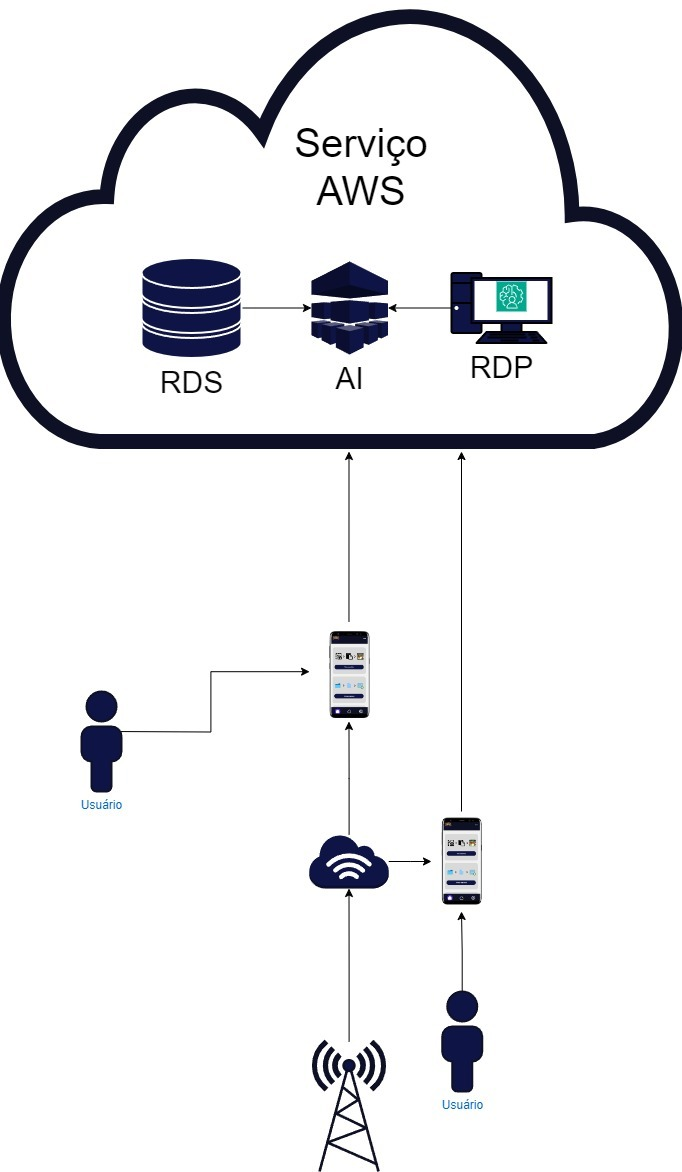
\includegraphics[scale=0.5]{Illustrations/Diagrama_redes.jpg}}
        \usebox0%
        \SourceOrNote{Autoria Própria (2024)}
    \end{figure}

    \textbf{Modelo de Negócios}
    
    Este é um modelo de Business Model Canvas para um aplicativo voltado para a identificação da bacteriose Xanthomonas Phaseoli nas folhas de mandioca, focado principalmente nos agricultores do Vale do Ribeira. 

    Parcerias Chave

    No contexto do projeto, as parcerias chaves incluem pequenmos agricultores locais que visam utilizar da tecnologia para melhorar a qualidade do serviço e também do produto; juntamente da Secretaria de Agricultura dos municípos do Vale do Ribeira. 

    Atividades Chave

    A principal atividade do projeto AVASS é fornecer uma solução automatizada e precisa para identificar a bacteriose nas folhas da mandioca de maneira eficiente e rápida, a fim de minimizar perdas nas colheitas.

    Proposta de Valor

    O aplicativo oferece uma solução para identificar a presença da Xanthomonas Phaseoli nas folhas de mandioca, também possuindo a proposta de preservação da qualidade da mandioca, permitindo que os agricultores façam um monitoramento das áreas mais afetadas com auxilio de um mapa de calor.

    Relacionamento com o Cliente

    O aplicativo oferece suporte direto aos usuários, permitindo que eles descrevam o problema ocorrido e aguardem uma resposta da equipe de suporte; além disso, disponibiliza tutoriais para auxiliar na configuração e uso adequado do sistema, bem como um sistema de feedback onde os usuários podem relatar problemas e sugerir melhorias.

    Segmento de Mercado

    O público-alvo do aplicativo são agricultores de mandioca, especialmente aqueles que cultivam na região do Vale do Ribeira, os quais podem ser diretamente impactados pela bacteriose e, portanto, se beneficiarão do aplicativo para prevenção da bacteriose em suas plantações e suas possíveis perdas.

    Recursos Chave

    O projeto requer programadores para o desenvolvimento e manutenção do aplicativo, funcionários de assistência técnica para auxiliar agricultores e usuários na resolução de problemas técnicos, e uma infraestrutura de hospedagem para armazenamento seguro de dados e realização de análises de forma eficiente (AWS).

    Canais

    Os meios de acesso ao projeto incluem apresentações em feiras e eventos agrícolas, onde ele pode ser demonstrado, além de um site dedicado que atua como canal digital para divulgação e informações sobre o projeto, juntamente com anúncios direcionados ao público que busca soluções para problemas de bacteriose nas plantações de mandioca.

    Estrutura de Custo

    Custo de Manutenção: Inclui despesas gerais como energia e água; Desenvolvimento de Software: Custos relacionados ao desenvolvimento e atualização do aplicativo; Hospedagem: Manutenção de servidores para o site e o aplicativo; Equipamentos: Computadores, monitores, teclados e outros equipamentos necessários para a equipe técnica.

    Fontes de Renda

    O modelo de receita é baseado em assinaturas, onde os usuários pagam uma taxa mensal para acessar o serviço. Isso permite uma receita recorrente e sustentação do projeto. O usuário possuira um teste gratis contendo somente 3 análises, onde respectivamente ele pode tirar somente 3 fotos.

    \begin{figure}[b]
        \centering
        \SetCaptionWidth{\ifbool{@LayoutA}{0.6}{0.72}\linewidth}
        \caption{Modelo de Negócios}%
        \label{phot:pg-11}
        \savebox0{\includegraphics[scale=0.4]{Illustrations/Canva.jpg}}
        \usebox0%
        \SourceOrNote{Autoria Própria (2024)}
    \end{figure}
    
